% poster.tex
%
% Presentation of the work done for my Bachelor thesis. 
% The poster only deals with the mean field theory predicting the
% network activity
%
% To be presented on the conference "Computational Neuroscience and the Hybrid Brain", 
% October 12-14, 2015, Facultry of Biology, University Freiburg. 
%
% Friedrich Schuessler, 10.2015

\documentclass[portrait, final, a0paper, fontscale=0.34, leqno]{baposter}
%\documentclass[a4shrink,portrait,final]{baposter}
% Usa a4shrink for an a4 sized paper.

\tracingstats=2

\usepackage[utf8]{inputenc}
\usepackage{calc}
\usepackage{graphicx}
\usepackage{tabularx} %Tables
\usepackage{amsmath}
\usepackage{amssymb}
\usepackage{relsize}
\usepackage{multirow}
\usepackage{rotating}
\usepackage{bm}
\usepackage{url}

% Justify: Left alignment within multicols environment
\usepackage{multicol}
\usepackage{ragged2e} 
\usepackage{etoolbox}
\AtBeginEnvironment{multicols}{\RaggedRight}
% Columns of adjustable size:
\usepackage{vwcol} 

% Fonts
%\usepackage{times}
%\usepackage{helvet}
%\usepackage{bookman}
%\usepackage{palatino}
\usepackage{cmbright}

\usetikzlibrary{calc}
\graphicspath{{figures/}}
\DeclareGraphicsExtensions{.pdf,.png,.jpg, .eps}
\newcommand{\captionfont}{\footnotesize}

%%%%%%%%%%%%%%%%%%%%%%%%%%%%%%%%%%%%%%%%%%%%%%%%%%%%%%%%%%%%%%%%%%%%%%%%%%%%%%%%
% Additional (not from the template)
%%%%%%%%%%%%%%%%%%%%%%%%%%%%%%%%%%%%%%%%%%%%%%%%%%%%%%%%%%%%%%%%%%%%%%%%%%%%%%%%
\usepackage{smcaps} % costum style file: "smcaps.sty": small caps for cmbright
%\usepackage{pgfbaselayers}
%\pgfdeclarelayer{background}
%\pgfdeclarelayer{foreground}
%\pgfsetlayers{background,main,foreground}


%%%%%%%%%%%%%%%%%%%%%%%%%%%%%%%%%%%%%%%%%%%%%%%%%%%%%%%%%%%%%%%%%%%%%%%%%%%%%%%%
% Multicol Settings
%%%%%%%%%%%%%%%%%%%%%%%%%%%%%%%%%%%%%%%%%%%%%%%%%%%%%%%%%%%%%%%%%%%%%%%%%%%%%%%%
\setlength{\columnsep}{1em}
\setlength{\columnseprule}{0mm}


%%%%%%%%%%%%%%%%%%%%%%%%%%%%%%%%%%%%%%%%%%%%%%%%%%%%%%%%%%%%%%%%%%%%%%%%%%%%%%%%
% Save space in lists. Use this after the opening of the list
%%%%%%%%%%%%%%%%%%%%%%%%%%%%%%%%%%%%%%%%%%%%%%%%%%%%%%%%%%%%%%%%%%%%%%%%%%%%%%%%
\newcommand{\compresslist}{%
\setlength{\itemsep}{1pt}%
\setlength{\parskip}{0pt}%
\setlength{\parsep}{0pt}%
}

%%%%%%%%%%%%%%%%%%%%%%%%%%%%%%%%%%%%%%%%%%%%%%%%%%%%%%%%%%%%%%%%%%%%%%%%%%%%%%%%
% Math stuff
%%%%%%%%%%%%%%%%%%%%%%%%%%%%%%%%%%%%%%%%%%%%%%%%%%%%%%%%%%%%%%%%%%%%%%%%%%%%%%%%
\newcommand*\diff{\mathop{}\!\text{d}}
\newcommand*\Diff[1]{\mathop{}\!\text{d^#1}}

%%%%%%%%%%%%%%%%%%%%%%%%%%%%%%%%%%%%%%%%%%%%%%%%%%%%%%%%%%%%%%%%%%%%%%%%%%%%%%
%%% Begin of Document
%%%%%%%%%%%%%%%%%%%%%%%%%%%%%%%%%%%%%%%%%%%%%%%%%%%%%%%%%%%%%%%%%%%%%%%%%%%%%%

\begin{document}

%%%%%%%%%%%%%%%%%%%%%%%%%%%%%%%%%%%%%%%%%%%%%%%%%%%%%%%%%%%%%%%%%%%%%%%%%%%%%%
%%% Here starts the poster
%%%---------------------------------------------------------------------------
%%% Format it to your taste with the options
%%%%%%%%%%%%%%%%%%%%%%%%%%%%%%%%%%%%%%%%%%%%%%%%%%%%%%%%%%%%%%%%%%%%%%%%%%%%%%
% Define some colors
%colors =   [
            %"#08519c",
            %"#9ecae1",
            %"#a63603",
            %"#fdae6b",
            %"#54278f",
            %"#bcbddc",
            %"#006d2c",
            %"#a1d99b"
            %]
\definecolor{bgcolor}{HTML}{FFFFFF}
\definecolor{bgcolor2}{HTML}{FCDFC5}
\definecolor{bordercolor}{HTML}{A63603}
\definecolor{headercolor}{HTML}{FCCDA3}
\definecolor{headerfontcolor}{HTML}{000000}
\definecolor{boxcolor}{HTML}{FFFFFF}

%%
\typeout{Poster Starts}
%\background{
  %\begin{tikzpicture}[remember picture,overlay]%
    %\draw (current page.north west)+(-2em,2em) node[anchor=north west] {
\includegraphics[height=1.05\textheight]{drawing.pdf}};
  %\end{tikzpicture}%
%}

\newlength{\leftimgwidth}
\begin{poster}%
  % Poster Options
  {
  % Show grid to help with alignment
  grid=false,
  % Number of columns
  columns=2,
  % Column spacing
  colspacing=1em,
  % Color style
  bgColorOne=bgcolor,
  bgColorTwo=bgcolor2,
  borderColor=bordercolor,
  headerColorOne=headercolor,
  headerColorTwo=white, % only for gradients
  headerFontColor=headerfontcolor,
  boxColorOne=boxcolor,
  boxColorTwo=white,    % only for gradients
  % Format of textbox
  textborder=roundedsmall,
  % Format of text header
  eyecatcher=false,
  headerborder=open, 
  headerheight=0.1\textheight,
  headershape=smallrounded,
  headershade=plain,
  headerfont=\Large\textsf, %Sans Serif
  boxshade=plain,
  background=shadetb,
  %background=user,
  linewidth=2pt
  }
  % Eye Catcher
  {\includegraphics[width=10em]{D1077}} % No eye catcher for this poster. (eyecatcher=no above). If an eye catcher is present, the title is centered between eye-catcher and logo.
  % Title
  {\sf %Sans Serif
  %\bf% Serif
      A Mean Field Theory for a layered Network Model of the Neocortex
\vspace{0.3em}}
  % Authors
  {\sf %Sans Serif
  % Serif
      \vspace{0em}\Large{Friedrich Schuessler\,$^{1}$, Benjamin Merkt\,$^{2}$, Stefan Rotter\,$^{2}$\\
  \normalsize
  $^1$\,Faculty of Physics, University of Freiburg -- 
  $^2$\,Bernstein Center Freiburg and Faculty of Biology, University of Freiburg 
  }
  }
  % University logo
  {% The makebox allows the title to flow into the logo, this is a hack because of the L shaped logo.
    \makebox[8em][r]{%
      \begin{minipage}{16em}
        \hfill
        
\includegraphics[height=10em]{unisiegel}
      \end{minipage}
    }
  }

%%%%%%%%%%%%%%%%%%%%%%%%%%%%%%%%%%%%%%%%%%%%%%%%%%%%%%%%%%%%%%%%%%%%%%%%%%%%%%
%%% Now define the boxes that make up the poster
%%%---------------------------------------------------------------------------
%%% Each box has a name and can be placed absolutely or relatively.
%%% The only inconvenience is that you can only specify a relative position 
%%% towards an already declared box. So if you have a box attached to the 
%%% bottom, one to the top and a third one which should be in between, you 
%%% have to specify the top and bottom boxes before you specify the middle 
%%% box.
%%%%%%%%%%%%%%%%%%%%%%%%%%%%%%%%%%%%%%%%%%%%%%%%%%%%%%%%%%%%%%%%%%%%%%%%%%%%%%


%%%%%%%%%%%%%%%%%%%%%%%%%%%%%%%%%%%%%%%%%%%%%%%%%%%%%%%%%%%%%%%%%%%%%%%%%%%%%%
\headerbox{MOTIVATION}{name=motivation, column=0, span=2}{
    \begin{multicols}{2}
    Current research on the function of the neocortex 
    \end{multicols}
}


%%%%%%%%%%%%%%%%%%%%%%%%%%%%%%%%%%%%%%%%%%%%%%%%%%%%%%%%%%%%%%%%%%%%%%%%%%%%%%
\headerbox{SPIKING NETWORK MODEL}{name=network, column=0, span=1, below=motivation}{
    \centerline{\uppercase{Global network structure}}
    \vspace{0.2cm}
    8 populations are arranged in 4 layers, each containing an excitatory and 
    inhibitory population. Neuron and synapse numbers are estimated from 
    experimental data by Potjans and Diesmann. Synapses are drawn randomly until 
    a fixed number is reached. Both synapse weights and delays are drawn from Gaussian
    distributions. There's no plasticity. Each neuron receives independent Poissonian 
    spikes as input. Both spike times and membrane potentials are measured. 

    \begin{multicols}{3}
        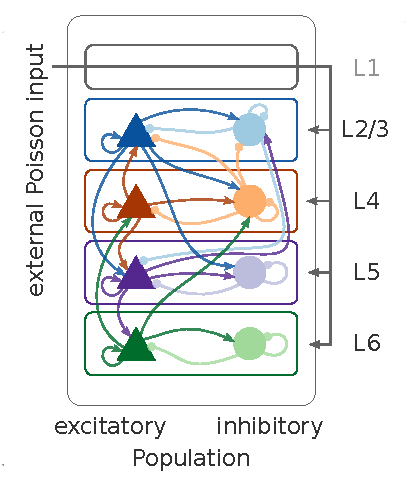
\includegraphics[height=5.0cm]{diagram} 
        \columnbreak

        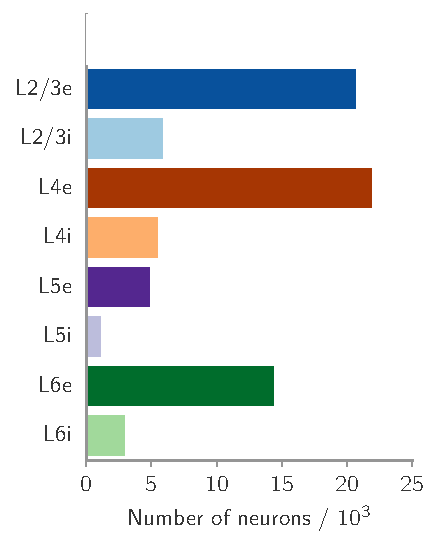
\includegraphics[height=5.0cm]{population_size} 
        \columnbreak
        
        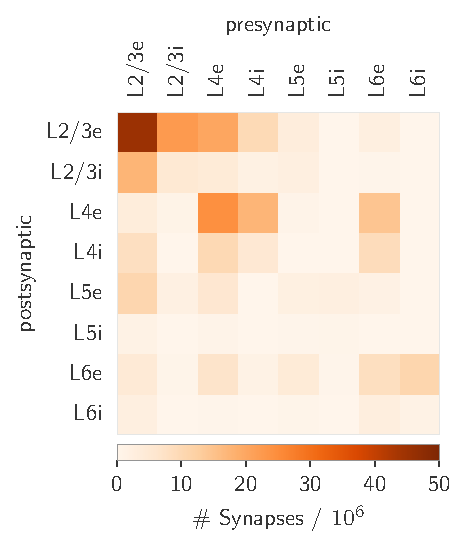
\includegraphics[height=5.0cm]{synapse_numbers} 
    \end{multicols} 
    %\vspace{0.4cm}

    \centerline{\uppercase{Leaky integrate-and-fire neuron}}
    \vspace{0.2cm}
    \begin{vwcol}[widths={0.75, 0.3},
            sep=.4cm, rule=0pt, indent=0em] 
    \setcounter{equation}{0}
    Membrane potentials $V_i$ are modeled as an RC circuit:
        \begin{equation}
            \tau_\text{m} \,\frac{\text{d} V_i(t)}{\text{d} t} 
            = - (V_i(t) - E_L) + \frac{\tau_\text{m}}{C_\text{m}} I_i(t) \,.
            \label{eq:lif-neuron}
        \end{equation}
        If $V_i(t)$ reaches the threshold $\theta$: \\
        \vspace{0.2cm}
            \quad $\Rightarrow$ 
                Spike is emitted \\
        \vspace{0.2cm}
            \quad $\Rightarrow$ 
                $V_i(t) = E_L$ \,for refractory period $\tau_\text{rp}$ 

    
\includegraphics[width=2cm]{RC_circuit}

    \end{vwcol} 

    \vspace{0.5cm}
    \centerline{\uppercase{Current-based synapse model}}
    \vspace{0.3cm}
    Each spike of neuron $j$ elicits an exponentially decaying current in the
    postsynaptic neuron~$i$.  
    The amplitude is set by the synaptic weight $w_{ij}$. 
    The total incoming current is a sum over all synapses:
    \begin{equation}
        I_i(t) = 
            \sum_j w_{ij} \sum_k 
            \exp\left(\frac{t - t_j^k - d_{ij}}{\tau_\text{syn}}\right) ,
    \end{equation}
    where $t^k_j$ is the spike time of the $k$-th spike of neuron $j$.
}


%%%%%%%%%%%%%%%%%%%%%%%%%%%%%%%%%%%%%%%%%%%%%%%%%%%%%%%%%%%%%%%%%%%%%%%%%%%%%%
\headerbox{MEAN FIELD THEORY}{name=meanfield, column=0, span=1, below=network}{
    The mean field model predicts firing rates for spiking network models of 
    leaky integrate-and-fire neurons (Equation \eqref{eq:lif-neuron}).
    For a sparsely connected network with uncorrelated input to each neuron, 
    the input current $I_i(t)$ to neuron $i$ in population $a$ can be described by 
    the stochastic equation
    \begin{align}
        \frac{\tau_\text{m}}{C_\text{m}} \, I_i(t) &= 
            \mu_a(t) + \sigma_a(t) \sqrt{\tau_\text{m}} \eta_i(t) \\
    \intertext{
    with average part $\mu$ and amplitude $\sigma$
    of the Gaussian white noise $\eta_i$ :
    }
        \mu_a        &= 
            \tau_\text{m}
            \sum_{b \,\in \text{pop.}} C_{ab} \, J_{ab} \, \nu_b +
            \tau_\text{m} C^\text{ext}_a J  \nu_\text{ext} 
            \, ; \\
        {\sigma_a}^2 &= 
            \tau_\text{m} 
            \sum_{b \,\in \text{pop.}} C_{ab} \, {J_{ab}}^2  \, \nu_b + 
            \tau_\text{m} C^\text{ext}_a J^{2} \nu_\text{ext} \,.
    \end{align}
    Transformation via
    \begin{enumerate}
        \item 
        $\Rightarrow$ Fokker--Planck eq. for membrane potential distributions; 
        \item 
        $\Rightarrow$ stationary solution to Fokker--Planck eq.;
        \item 
        $\Rightarrow$ normalization condition for probability distributions
    \end{enumerate}
    leads to a self-consistency equation for the firing rates $\nu_a$ of each population:
    \begin{equation}
        \frac{1}{\nu_{a}} = \tau_{rp} 
            + \tau_\text{m} \sqrt{\pi}
            \int_{\frac{V_\text{r} - \mu_{a}}{\sigma_{a}}}^{\frac{\theta - \mu_{a}}{\sigma_{a}}} 
            e^{u^2} \left(1 + \text{erf}(u)\right) \diff u \,.
        \label{eq:self-consistency}
    \end{equation}
    The equations are coupled via the integral boundaries. Solutions are found
    numerically. 
}


%%%%%%%%%%%%%%%%%%%%%%%%%%%%%%%%%%%%%%%%%%%%%%%%%%%%%%%%%%%%%%%%%%%%%%%%%%%%%%
\headerbox{RESULTS}{name=results, column=1, span=1, below=motivation}{
\begin{minipage}{0.98\linewidth}
    \centerline{\uppercase{Firing rates and Irregularity}}
    %\vspace{0.1cm}
    \begin{multicols}{3}
        \includegraphics[height=5cm]{results_rates}  
        \columnbreak 
        \columnbreak \\
        Comparison of theoretical predictions 
        to corresponding measures from 20 independent simulations (crosses). 
        The firing rates are calculated according to 
        Equation \eqref{eq:self-consistency}.
        Irregularity is measured by the coefficient of variation of interspike intervals
        of single neurons.\\
    \end{multicols}
        
    \centerline{\uppercase{Membrane potential distributions}}
    %\vspace{0.1cm}
    \begin{multicols}{3}
        \includegraphics[width=8cm]{results_membrane} 
        \columnbreak 
        \columnbreak \\
        The theoretical values (smooth curves)
        correspond to the steady state solutions of the Fokker--Planck equations. 
        The effect of neurons coming out from the refractory period at -65 mV can
        be observed both in the data and the theoretical prediction.
    \end{multicols}
        
    \centerline{\uppercase{Exploring the parameter space}}
    %\vspace{0.1cm}
    \begin{multicols}{3}
        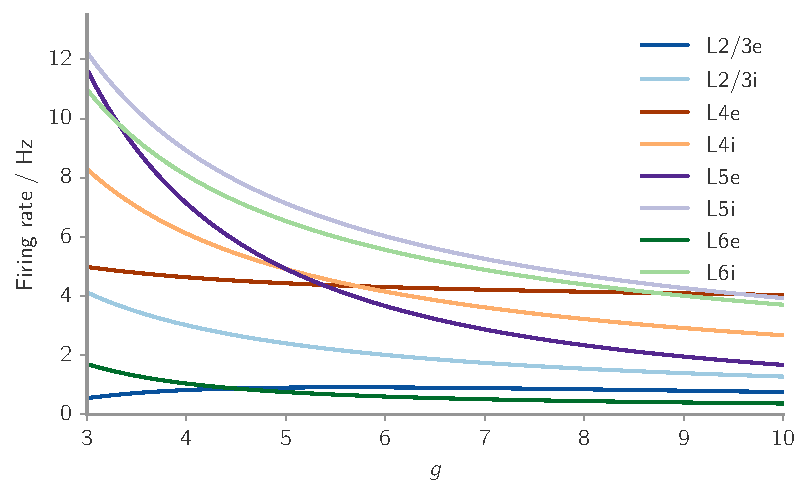
\includegraphics[width=8cm]{simulate_change_g} 
        \columnbreak 
        \columnbreak \\
        Firing rates are predicted for varying $g$, 
        governing the ratio of inhibition over excitation. The previous working point 
        was at global balance, $g=4$. Simulating a comparable
        number of data points would take several days, the prediction is done in seconds.
    \end{multicols}
\end{minipage}
}


%%%%%%%%%%%%%%%%%%%%%%%%%%%%%%%%%%%%%%%%%%%%%%%%%%%%%%%%%%%%%%%%%%%%%%%%%%%%%%
\headerbox{CONCLUSION}{name=conclusion, column=1, span=1, below=results}{
    \begin{itemize}
        \item The mean field theory predicts firing rates and irregularity 
            to a high accuracy (relative errors below 10\,\%). 
        \item Deviations may be due to neglecting correlations.
        \item The theory can be applied as a convenient computational tool
            (large advantages in terms of computational time over simulations).
    \end{itemize}
}

%%%%%%%%%%%%%%%%%%%%%%%%%%%%%%%%%%%%%%%%%%%%%%%%%%%%%%%%%%%%%%%%%%%%%%%%%%%%%%
\headerbox{VARIABLES}{name=variables, column=1, span=1, below=conclusion}{
    \begin{multicols}{2}
    \begin{tabular}{>{$}p{1.0cm}<{$} p{4.5cm}}
        \multicolumn{2}{l}{\uppercase{Spiking network model}} \\[0.08cm]
        V_i(t)          &  Membrane potential  \\
        E_L             &  Resting potential  \\
        \tau_\text{m}   &  Membrane time constant \\ 
        C_\text{m}      &  Membrane capacity  \\
        I_i(t)          &  Input current       \\
        \tau_\text{syn} & Synaptic time constant \\
        w               & Synaptic strength \\
        d               & Delay
    \end{tabular} 
    \columnbreak
    \begin{tabular}{>{$}p{1.0cm}<{$} p{4.5cm}}
        \multicolumn{2}{l}{\uppercase{Mean field model}}\\ [0.08cm]
        \multicolumn{2}{l}{Recurrent (populations $a$ and $b$):}\\
        C_{ab}          & Synapse number\\ 
        J_{ab}          & Synaptic weight\\ 
        \nu_a           & Single neuron firing rate\\
        \multicolumn{2}{l}{External:}\\
        C^\text{ext}_{a}& Synapse numbers\\ 
        J               & Synaptic weight *\\ 
        \nu_\text{ext}  & Rate of Poisson process
    \end{tabular} 
    \end{multicols}
    * Synapses are modeled differently: 
    Whereas the spiking network model uses current based exponential synapses, 
    the mean field theory is originally developed for voltage based delta synapses.
    To include the difference, $J$ can be adapted.
}
    

%%%%%%%%%%%%%%%%%%%%%%%%%%%%%%%%%%%%%%%%%%%%%%%%%%%%%%%%%%%%%%%%%%%%%%%%%%%%%%
\headerbox{REFERENCES}{name=references,column=1,above=bottom}{
    \smaller
    \bibliographystyle{ieee}
    \renewcommand{\section}[2]{\vskip 0.05em}
      \begin{thebibliography}{1}\itemsep=-0.01em
      \setlength{\baselineskip}{0.4em}
      \bibitem{brunel2000:dynamics}
        N.~Brunel.
        \newblock 
            {D}ynamics of sparsely connected networks of excitatory and inhibitory 
            spiking neurons.
        \newblock 
        \textit{{J}ournal of computational neuroscience}, 2000
      \bibitem{potjans2014:microcircuit}
        T.~Potjans and M.~Diesmann.
        \newblock 
            {T}he cell-type specific cortical microcircuit: {R}elating structure and
            activity in a full-scale spiking network model.
        \newblock 
            \textit{{C}erebral Cortex}, 2014
      \end{thebibliography}
   \vspace{0.3em}
  }


%%%%%%%%%%%%%%%%%%%%%%%%%%%%%%%%%%%%%%%%%%%%%%%%%%%%%%%%%%%%%%%%%%%%%%%%%%%%%%%
  %\headerbox{ACKNOWLEDGEMENTS}{name=acknowledgements,column=1,above=bottom}{
%%%%%%%%%%%%%%%%%%%%%%%%%%%%%%%%%%%%%%%%%%%%%%%%%%%%%%%%%%%%%%%%%%%%%%%%%%%%%%
    %Still?
%}

\end{poster}%
\end{document}
